\subsection{Primordial Black Holes}
Primordial Black Holes (PBH) are hypothetical black holes thought to have formed in the early universe due to the gravitational collapse of highly dense regions. Since these black holes don't have the usual star as a progenitor, their masses can be lower than the actual mass required for forming a normal black hole. They were first theorized by Yakov Barisovich Zel'dovich and Igor Dmitriyevich Novikov in 1966, and theories of their origin were studied by Stephen Hawking in 1971. \cite{PBH_defn}

\begin{wrapfigure}{r}{5.5cm}
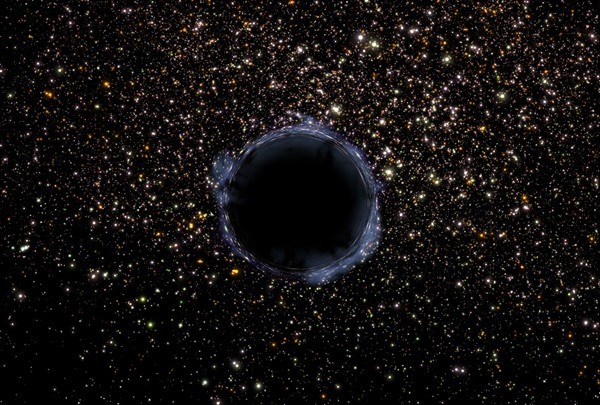
\includegraphics[width=5.5cm]{images.tex/pbh.jpg}
\caption{Computerized image of a primordial black hole.\\
    Source:-\url{https://astronomy.com/news/2019/07/primordial-black-holes}}
\end{wrapfigure} 

\subsubsection{PBH and Stochastic Gravitational Waves}
In the early universe, quantum fluctuations made the inflaton field highly unstable and non-uniform. In rare cases, these fluctuations might have spiked high enough to form energetic peaks which then collapse to form PBHs. This phenomenon would also result in the generation of a stochastic GW (discussed in the next section) background. But, to form such a background, a sufficient number of PBHs are required, which is only possible if the amplitude of the fluctuations are high enough at small scales. \cite{Nakama_2017}\\

Related with PBH and stochastic GW is the concept of cosmic horizon reentry. As the universe expands, represented by the scale fact $a$, comoving length scales\footnote{Comoving length scales/distances are the measure of distances between fundamental observers, i.e, observers that are moving with the expansion of the universe (Hubble Flow), and doesn't change with time.}  between two objects grow along with it. During inflation, $a$ grows exponentially, $a(t) \sim e^{Ht}$, where H is the Hubble constant. But, the horizon stays nearly constant during inflation. Now, the quantity $aH = \dot{a}$ tells us, through its variations in time, whether the comoving length scales grow at a greater or lesser rate than the horizon. During inflation, $a\dot{H} = \ddot{a} > 0$, so the comoving scales grow larger than the Hubble horizon, and after inflation, $a\dot{H} = \ddot{a} < 0$, so the horizon overtakes the comoving lengths, thus an object which was moved outside the horizon during inflation is back inside the horizon. This phenomenon is called Cosmic Horizon Reentry.\\

The survival of oscillation modes of the inflaton field depend on this phenomenon. The modes which leave the horizon and reenter it undergo a 'classical-to-quantum' transition, which transform them into curvature perturbations. These are the perturbations which have the chance to get highly energetic and yield PBH and the stochastic GW. The modes which never leave the horizon don't undergo the transition, so they don't have a major impact on the inflaton field. \cite{CHE}

\subsubsection{PBH and Gravitational Wave Bursts}
If in a small region, numerous curvature perturbations collapse, then a cluster of PBH could form. They dynamics of such PBH is completely different from that of binary PBH systems. Instead of ending up in traditional bound systems and spiral in, majority of PBHs in a cluster would produce a single scattering event via a hyperbolic encounter, only if their relative velocity or relative distance is high enough to escape getting captured into bound systems. Such events would produce bursts of GWs, which can be detected up to several Gpc. \\

In hyperbolic encounters, majority of the energy is released near the closest approach. This has a characteristic peak frequency, which mainly depends on the impact parameter $b$, the eccentricity $e$ and the total mass of the system $M$. These encounters has a duration of the order of a few milliseconds to several hours. GWs from such encounters have very different properties and signature when compared to those from traditional binaries, so detecting them would strengthen the possibility of the existence of PBH. \cite{Garc_a_Bellido_2017}
\pagebreak
